

\subsection{Architektur und Zusammenarbeit der Komponenten}        
\label{sec:Architektur und Zusammenarbeit der Komponenten-1} 

Mithilfe der Technologien und Softwarelösungen, die in Kapitel \ref{sec:Theorie-1} erläutert worden sind, und der Hardware, die in Kapitel \ref{sec:Beschreibung der Hardware-1} vorgestellt wurde, konnten die verschiedenen Komponenten, die bereits in der Aufgabenstellung (vgl. Kapitel \ref{sec:Aufgabenstellung-1}) genannt worden sind, umgesetzt werden. 
Im folgenden soll ein Überblick über die Zusammenarbeit der einzelnen Komponenten gegeben werden, bevor in den folgenden Kapiteln auf die genaue Entwicklung der einzelnen Komponenten eingegangen wird. 

Für den Nutzer gibt es ein Webfrontend, welches mithilfe eines Nginx Webservers (vgl. Kapitel {sec:WebserverNginx-1}) realisiert wird. Dieses Webfrontend greift auf ein \ac{REST} \ac{API}-Backend zurück, welches in \ac{PHP} geschrieben wurde und ebenfalls über den Nginx realisiert wird. Mithilfe dieses Backends werden die verschiedenen \ac{API} Routen realisiert, die dann den Zugriff auf die Datenbank organisieren. Das Backend besteht ebenfalls aus einigen Skripten, die in Python\ref{src:Python-1}) geschrieben sind. Diese Skripte organisieren die Kommunikationsendpunkte für die Buttons, indem sie auf die entsprechende Kommunikationsports für die Datenpakete lauschen und die Daten dann verarbeiten. 

Neben der Kommunikation wird ebenfalls ein Teil der \ac{REST} \ac{API} in Python realisiert. Dieser Teil ermöglicht sowohl den Status der Skripte, die die Kommunikation organisieren, abzufragen als auch die Skripte neu zu starten, sollte ein Skript nicht gestartet sein oder ein Fehler aufgetreten sein. Diese Daten werden ebenfalls für das Webfrontend verwendet. 
Die Buttons, als weitere Komponente, werden durch verschiedene Hardwareelemente realisiert. Mithilfe entsprechender Programme, die auf die Controller geladen werden, stellen sie eine Verbindung zu den definierten Kommunikationspunkten her. Über dieses Kommunikationsprotokoll werden dann, sobald der Button betätigt wurde, die entsprechenden Daten gesendet und dann im Backend verarbeitet. 
Zur Verarbeitung der Daten gehört auch das Einfügen in die entsprechenden Tabellen der SQL Datenbank, die auf einem MySQL Datenbankserver läuft, der für die Verwaltung der Daten zuständig ist. 
% Vielleicht noch ein passendes Modell einfügen


\newpage

\subsection{Entwicklung der Buttons}  
\label{sec:Entwicklung der Buttons-1} 

Im folgenden soll auf die Entwicklung der Button Komponente im Projekt eingegangen werden. Dabei wird insbesondere auf die Programmierung und Umsetzung eingegangen werden. 
Bei der Entwicklung der verschiedenen Buttons wurde insbesondere darauf geachtet, dass verschiedene Technologien getestet werden, um möglichst viele technische Möglichkeiten zu untersuchen. Das ist damit zu begründen, dass das Untersuchen von möglichst vielen Möglichkeiten zum Projektziel gehörte. 

\subsubsection{Entwicklung mit dem ``Pretzelboards''}  
\label{sec:Entwicklung mit dem ``Pretzelboards''-1}
\begin{figure}[!htb]
	\centering
	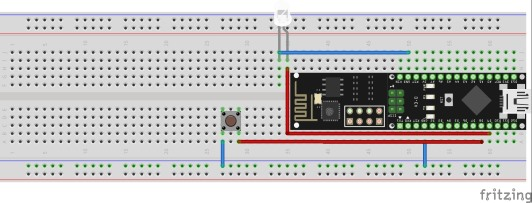
\includegraphics[scale=1.5]{Pretzel_Fritzing.jpg}
	\caption[Pretzelboard Versuchsaufbau]{Pretzelboard Versuchsaufbau,\\ Quelle: Eigener Entwurf mit Hilfe des Tools Fritzing (vgl. \cite{.fritz})}
\end{figure}

\subsubsection{Entwicklung mit dem ESP8266 Lua}  
\label{sec:Entwicklung mit dem ESP8266-1}
Die Entwicklung mit dem ESP Board verlief analog wie die mit dem Pretzel Board, jedoch wurden hier andere Ansätze ausprobiert.

Beispielsweise wurde der Code aufgrund seiner Kompaktheit nicht in Unterprozeduren unterteilt.
Dennoch wird in der "`setup"' Prozedur ebenfalls eine Verbindung mit dem \ac{WLAN} Netzwerk hergestellt, jedoch mit der Bibliothek ESP8266WiFi.h.
In der "`loop"' Prozedur wird ebenfalls der Status des Buttons überprüft, wenn dieser gedrückt wird, wird ein \ac{TCP} Client erzeugt, welcher sich mit dem Raspberry Pi verbindet, seine ID sendet und je nach Antwort und mitgeteiltem Status dann entweder eine grüne oder eine rote LED leuchten lässt. Grün bei erfolgreicher Übertragung und Rückmeldung des Servers; Rot im Falle eines Fehlers (vgl. Anhang \ref{sec:CodeESP}).
\begin{figure}[H]
	\centering
	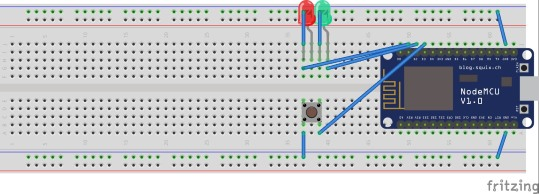
\includegraphics[scale=1.5]{ESP_Fritzing.jpg}
	\caption[ESP8266 Versuchsaufbau]{ESP8266 Versuchsaufbau,\\ Quelle: Eigener Entwurf mit Hilfe des Tools Fritzing (vgl. \cite{.fritz})}
\end{figure}

\subsubsection{Einbindung des Amazon Dash Buttons}  
\label{sec:Einbindung des Amazon Dash Buttons-1}
Bei der Einbindung des Amazon Dash Buttons galt es auf verschiedene Punkte zu achten. 
Da die Empfangsadresse der Pakete des Amazon Dash Buttons nicht verändert werden kann, galt es eine Möglichkeit zu finden, um den Druck auf den Button zu registrieren.
Eine Lösungsmöglichkeit wurde im mitlesen und scannen der Datenpakete gesehen, die der Amazon Dash Button an einen Server schicken muss, um die Bestellung aufzugeben.

Mithilfe des Tools tcpdump (vgl. \cite{.tcpdump}) wurde daher der Netzwerkverkehr mitgelesen, um die Verbindungen des Amazon Dash Buttons zu untersuchen. 
Bei dieser Untersuchung ist aufgefallen, dass die Kommunikation des Amazon Dash Buttons mit den Servern von Amazon zu großen Teilen verschlüsselt ist und daher nur wenige Informationen aus dem Mitlesen des Netzwerkverkehrs gewonnen werden konnten. 
Darunter fällt auch, dass keine eindeutige \ac{IP} Adresse erkannt werden konnte, an die die Nachrichten geschickt wurden, da die \ac{IP} Adressen, die ausgelesen wurden, in unregelmäßigen Abständen unterschiedlich waren.
Aufgrund dieser Ergebnisse konnte das Fazit gezogen werden, dass das Abfangen von \ac{TCP} bzw. \ac{HTTP} Daten keinen Erfolg versprach.
Daher wurde beschlossen eine andere Methode in Betracht zu ziehen.

Aufgrund der Tatsache, dass jedes Gerät im Netzwerk eine \ac{IP} Adresse im Netzwerk besitzt und diese angefodert werden muss, wurde das Mitlesen von \ac{ARP} Paketen in Betracht gezogen.
Mithilfe des Tools tcpdump konnte erneut der Netzwerkverkehr mitgeschnitten werden, allerdings wurde diesmal die Auswahl auf das Protokoll \ac{ARP} begrenzt. 
Bei dieser Untersuchung konnte erfolgreich der Amazon Dash Button identifiziert werden, da bei jedem Druck auf den Button zwei \ac{ARP} Pakete mitgelesen wurden.
Eines dieser Pakete ging vom Amazon Dash Button zum Raspberry Pi und eines zurück. 
Dieser Test wurde mehrmals wiederholt, unter anderem auch das Szenario, wenn der Button unmittelbar hintereinander gedrückt wird. 
Auch dieser Test war erfolgreich und die Pakete konnten erkannt werden.
Aufgrund dieser Ergebnisse wurde beschlossen, ein entsprechendes Python Skript als Serverskript zu entwickeln, welches diese Ergebnisse nutzt.
Die Entwicklung dieses Skript ist in Kapitel \ref{sec:Entwicklung des ARP Skripts-1} beschrieben. 
% bitte hier einbinden, dass es mithilfe eines entsprechenden Pythonscript und ifabfragen auf die MAC Adresse möglich wäre, dass man diese Buttons wirklich einsetzen könnte (stimmt doch?) 

\newpage

\subsection{Entwicklung des Frontends}  
\label{sec:Entwicklung der Frontends-1} 

\subsubsection{Aufbau und Entwicklung des Frontends}  
\label{sec:Aufbau und Entwicklung des Frontends-1}

\newpage

\subsection{Entwicklung und Einrichtung des Backends}  
\label{sec:Entwicklung und Einrichtung des Backends-1} 

In den folgenden Kapiteln wird auf die Einrichtung des Backends eingegangen. Dies umfasst sowohl die Einrichtung des Raspberry Pis, den Aufbau und die Entwicklung der REST API und die Entwicklung der Python Skripte. Die Einrichtung des Raspberry PIs wird an dieser Stelle geführt, da er das zentrale Hardwareelemente im Backend ist, da er genutzt wird, um die entsprechende Softwaredienste zur Verfügung zu stellen. Er stellt den zentralen Kommunikationspunkt im Projekt dar, da die Buttons nur ihn kennen, sich aber nicht gegenseitig. 

\subsubsection{Einrichtung des Raspberrys}  
\label{sec:Einrichtung des Raspberrys-1}

Die Einrichtung des Raspberry PIs besteht aus mehreren Schritten an dessen Ende die Verwendung des Raspberrys als zentraler Server steht. Die verschiedenen Schritte werden im folgenden erklärt: 
\paragraph{Einrichtung des Nginx}  
\label{sec:Einrichtung des Nginx-1} 

\paragraph{Einrichtung des SQL Datenbankservers}  
\label{sec:Einrichtung des SQL Datenbankservers-1} 

\paragraph{Einrichtung des WLAN Access Points}  
\label{sec:Einrichtung des WLAN Access Points-1} 

\paragraph{Einrichtung des UDP Empfängers}  
\label{sec:Einrichtung des UDP Empfängers-1} 

\paragraph{Einrichtung des TCP Empfängers}  
\label{sec:Einrichtung des TCP Empfängers-1} 


\subsubsection{Aufbau und Entwicklung der Python Skripte}  
\label{sec:Aufbau und Entwicklung der Python Skripte-1}

Mithilfe der Skriptsprache Python werden die verschiedenen Kommunikationsendpunkte in Form von Sockets realisiert. Um eine bessere Übersichtlichkeit zu gewährleisten und eine zentrale Verwaltung zu haben, gibt es ein Verwaltungsskript. Dieses Skript startet die anderen Skripte, die sich um jeweils einen Kommunikationsprotokoll kümmern. So gibt es ein Skript für die Kommunikation über \ac{UDP}, eins für \ac{TCP} und eins für \ac{ARP}, welches für die Amazon Dash Buttons genutzt wird. Aus diesen Gründen gibt es insgesamt vier Python Skripte, die einen wesentlichen Teil des Backends ausmachen.

\paragraph{Entwicklung des Verwaltungsskripts}$\;$ \\  
\label{sec:Entwicklung des Verwaltungsskripts-1} 
Das Verwaltungsskript dient, wie bereits erwähnt, als zentrales Skript, welches als einziges Skript auch gestartet werden muss. Über dieses Skript werden dann alle anderen notwendigen Skripte gestartet, die dann dafür sorgen, dass die Kommunikation ermöglicht wird. 
Neben dieser Funktionalität wird durch das Verwaltungsskript auch eine \ac{REST} \ac{API} realisiert. Diese wird mithilfe des Frameworks Flask (vgl. \cite{.s}) umgesetzt. Diese \ac{API} wird dazu genutzt, um einige Funktionalitäten bereitzustellen, die im Frontend benötigt werden. Als Beispiel wäre der aktuelle Status der Empfängerskripte (vgl. Kapitel \ref{sec:Entwicklung des UDP Skripts-1}) zu nennen. 

Die genannte \ac{REST} \ac{API} kann dann im Verwaltungsskript auf andere Methoden zugegriffen werden, die dann weitere Funktionen umfassen. Die Rückgabewerte dieser Funktionen werden dann im \ac{JSON} Format an das Frontend der Anwendung weitergegeben und können dann dort weiter verarbeitet werden. So kann beispielsweise im Frontend angezeigt werden, dass alle Kommunikationsmöglichkeiten zur Verfügung stehen. 

\paragraph{Entwicklung des \ac{UDP} Skripts}$\;$ \\  
\label{sec:Entwicklung des UDP Skripts-1} 
Da die Übertragung der Datenpakete über das \ac{UDP} Protokoll ermöglicht werden soll, muss ein entsprechender Empfänger auf dem Raspberry PI vorhanden sein. Dieser Empfänger wird mithilfe eines Skriptes in Python realisiert.

Dieses Skript nutzt die Library ``Socket'' (vgl. \cite{.20.02.2017}), welches es ermöglicht ein Socket zu erstellen. Dieses Socket wird an eine \ac{IP} Adresse und einen Port gebunden und wird anschließend für alle eingehenden \ac{UDP} Pakete genutzt. In einer Endlosschleife, welche manuell unterbrochen werden kann, wird auf eingehende Pakete gewartet. Die Endlosschleife wird benötigt, da ein Button zu jedem Zeitpunkt betätigt werden kann und somit dauerhaft auf ankommende Pakete geachtet werden muss. 

Bei Eingang eines entsprechenden Pakets wird ein entsprechendes Request an die \ac{REST} \ac{API} geschickt. Da als Übertragungsart allerdings das \ac{UDP} Protokoll genutzt wird, kann dem Button keine Rückmeldung gegeben werden, ob der Eintrag in die Datenbank über die \ac{REST} \ac{API} erfolgreich war. Zudem kann auch kein allgemeines Feedback zurückgegeben werden. Auch bei anderen Fehlern kann dem Button keine Rückmeldung gegeben werden. 

Nach dem erfolgreichen Absenden der Anfrage an die \ac{REST} \ac{API} befindet sich das Skript für den \ac{UDP} Empfänger weiterhin in der Endlosschleife und wartet auf das nächste Datenpaket. 
Das Skript ist im Anhang unter \ref{sec:UDPAnhang} zu finden. 

\paragraph{Entwicklung des \ac{TCP} Skripts}$\;$ \\  
\label{sec:Entwicklung des TCP Skripts-1} 
Für alle Datenpakete, die über das Protokoll \ac{TCP} empfangen werden, muss ebenfalls ein Skript geschrieben werden, welches diese Datenpakete verarbeitet. Dabei wird genauso vorgegangen, wie beim Skript für \ac{UDP}. Der einzige Unterschied ist nach dem Absenden der Anfrage an die \ac{REST} \ac{API}. Das Skript für \ac{TCP} Datenpakete wartet nach dem Absenden der Anfrage auf die Bestätigung und schickt eine entsprechende Antwort zurück an den Button. Dieser verarbeitet ebenfalls die Antwort und kann mithilfe einer Lampe auf dem Steckbrett dem Nutzer ein visuelles Feedback geben. 
Das entsprechende Skript ist im Anhang unter \ref{sec:TCPAnhang} zu finden.

\paragraph{Entwicklung des \ac{ARP} Skripts}$\;$ \\  
\label{sec:Entwicklung des ARP Skripts-1} 
Da das Mitlesen der \ac{IP} Datenpakete des Amazon Dash Buttons nicht möglich war, wurde das mitschneiden der \ac{ARP} Datenpakete notwendig, wie bereits in Kapitel \ref{sec:Einbindung des Amazon Dash Buttons-1} beschrieben. 
Im Vergleich zu den Skripten, die in den Kapiteln \nameref{sec:Entwicklung des UDP Skripts-1} und \nameref{sec:Entwicklung des TCP Skripts-1} beschrieben sind, ist dieses Skript etwas anders aufgebaut. Es wird zwar ebenfalls die Library ``Socket'' genutzt, allerdings ist die Konfiguration des Sockets anders, damit \ac{ARP} Datenpakete gelesen werden können. 


Das Lesen dieser Datenpakete beschränkt sich allerdings auf das Erkennen der \ac{IP} Adresse, die das Paket abschickt bzw. empfängt. Nur diese Informationen werden benötigt, da die Funktionalität des Skript darauf beruht, dass jeder zweite \ac{ARP} Request eine entsprechende Anfrage an die \ac{REST} \ac{API} abschickt. Das nur jeder zweite Request eine entsprechende Anfrage abschickt, ist damit begründet, dass bei einem einzelnen Druck auf den Amazon Dash Button ein \ac{ARP} Paket von Button zum Router geschickt wird und ein Paket vom Router zum Button. Das bedeutet, dass für jeden Druck zwei Requests abgeschickt werden. Daher löst nur jedes zweite Paket eine Anfrage aus, die dann die Anzahl eines Produktes in der Datenbank erhöht. 

Dies wird durch einen entsprechenden Zähler im Skript umgesetzt, welcher bei eins startet und bei dem Wert zwei eine entsprechende Anfrage an die \ac{REST} \ac{API} abschickt. Nach dem Abschicken der Anfrage wird der Zähler wieder auf eins gesetzt. 
Durch eine Unterscheidung von \ac{MAC} Adressen, welche ebenfalls im \ac{ARP} Header mitgeschickt werden, ist es auch möglich, dass verschiedene Amazon Dash Buttons eingebunden werden. 
Allerdings benötigt diese Konfiguration einige manuelle Arbeit, da das Skript nur manuell zu bearbeiten ist. 
Das entsprechende Skript ist im Anhang unter \ref{sec:ARPAnhang} zu finden.

\newpage